\chapter{Desarrollo de infraestructura y servicios web}

  En \'este cap\'itulo se analiza la infraestructura sobre la que se apoya la herramienta de Author y su motor de
  renderizado. El objetivo es tener una visi\'on global del proyecto y definir una estrategia de implementaci\'on.

  Author es una aplicaci\'on web, que utiliza React para la interfaz de usuario, la API de
  Canvas de HTML para el editor 2D y Three.js como motor de renderizado para el editor de 3D. Las interacciones de
  usuario actualizan el estado local del cliente y se comunica con el API REST para persistir los cambios sobre
  los recursos en base de datos. Este flujo permite el dise\~no y prototipado de la prenda completamente en el
  cliente web, mientras que para las acciones m\'as costosas, como la simulaci\'on o renderizado offline de tejidos,
  se reserva al usuario un servidor que utiliza un servicio HPC de Seddi encarga de recibir, procesar y enviar la
  petici\'on a traves del sistema de cola de mensajes.

  \begin{figure}[H]
    \vspace{1cm}
    \centering
      \frame{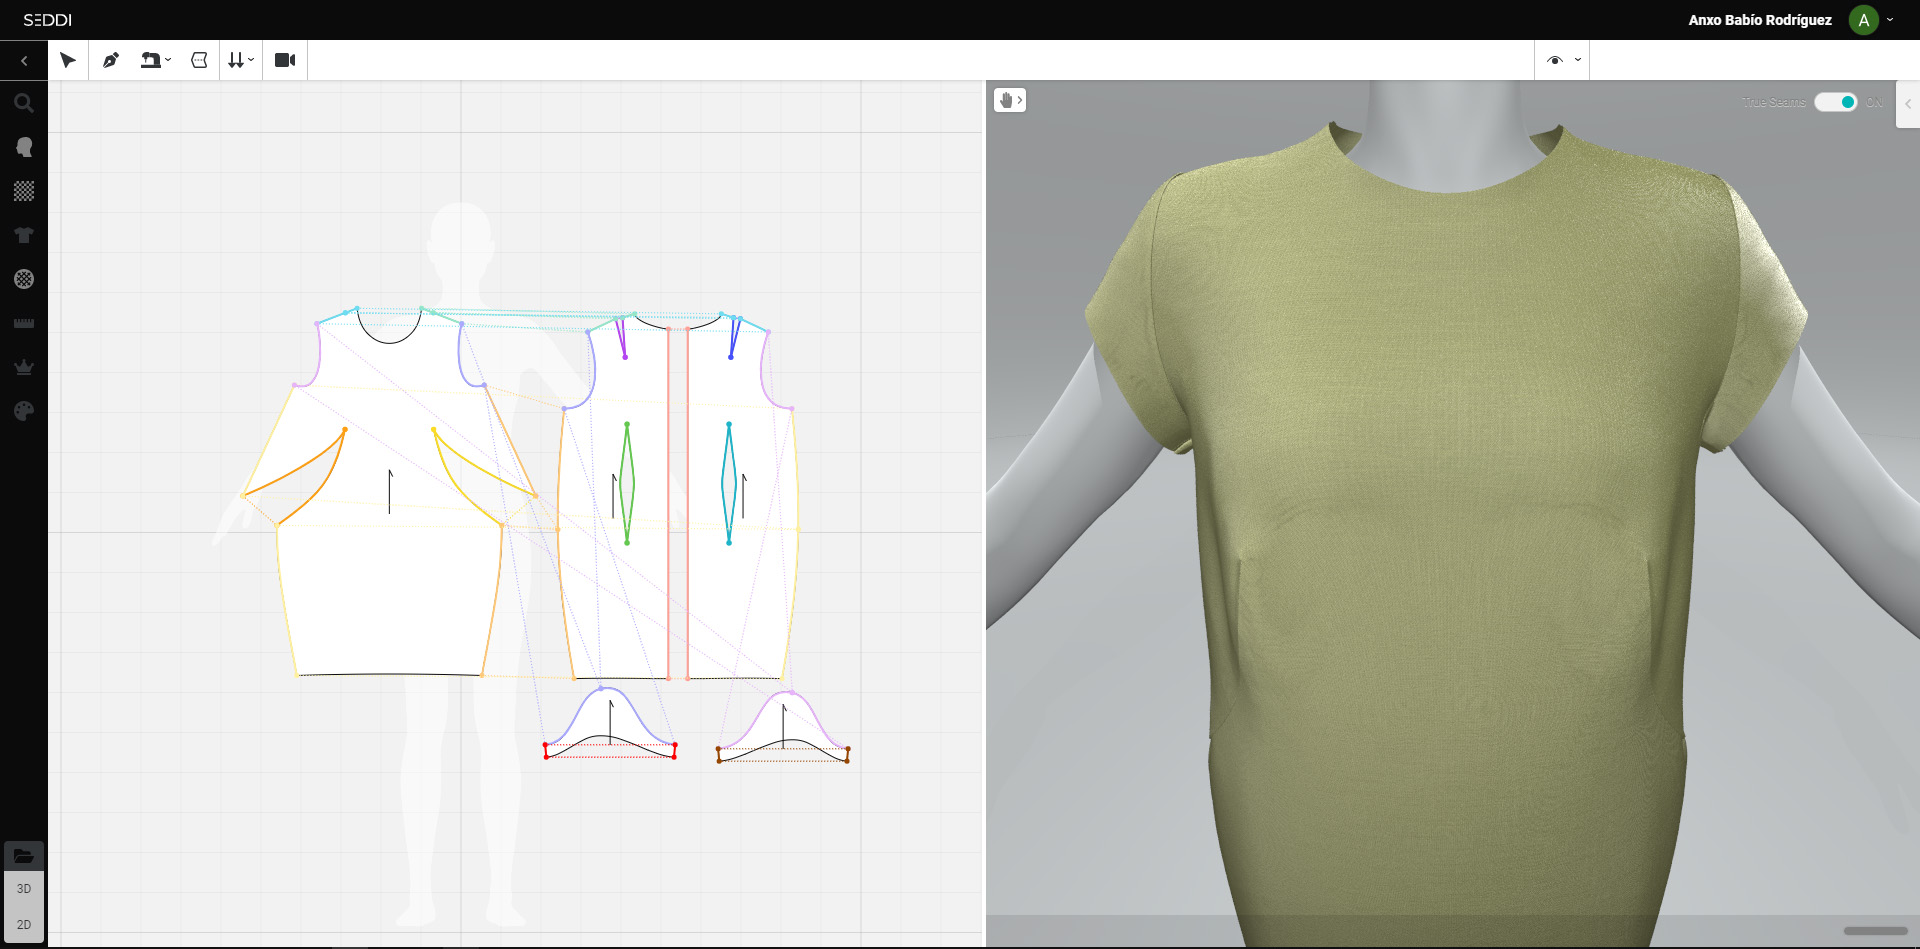
\includegraphics[scale=0.28]{viewports}}
    \caption{Editor de patrones 2D y editor 3D de Author}
    \vspace{0.5cm}
  \end{figure}

  \section{Servicios en la nube de Seddi}

  \bgroup

    Al contrario que en una arquitectura centralizada, en la que la l\'ogica de negocio se controla en un sistema
    principal, los servicios en la nube utilizan una arquitectura distribuida, diferentes servicios que se comunican
    entre s\'i para realizar una tarea en conjunto. Los servicios gestionan una colecci\'on de recursos relacionados
    y exponen su funcionalidad a trav\'es de contratos a otros usuarios y servicios parte del sistema. Este tipo de
    arquitectura implica una mayor complejidad, al tener que comunicar los diferentes servicios, pero ofrece una
    mayor escalabilidad, tolerancia a fallos y la posibilidad de compartir recursos entre las partes del sistema.

    Seddi ofrece sus servicios a trav\'es de clientes web que exponen la funcionalidad al usuario que se comunica con un API
    REST, para gestionar el acceso a recursos compartidos en la plataforma, y una conexion de sockets con un sistema de cola de
    mensajes para pedir y recibir en tiempo real las operaciones graficas mas costosas que se realizan en los servidores en la nube.

    \begin{figure}[H]
      \vspace{1cm}
      \centering
        \frame{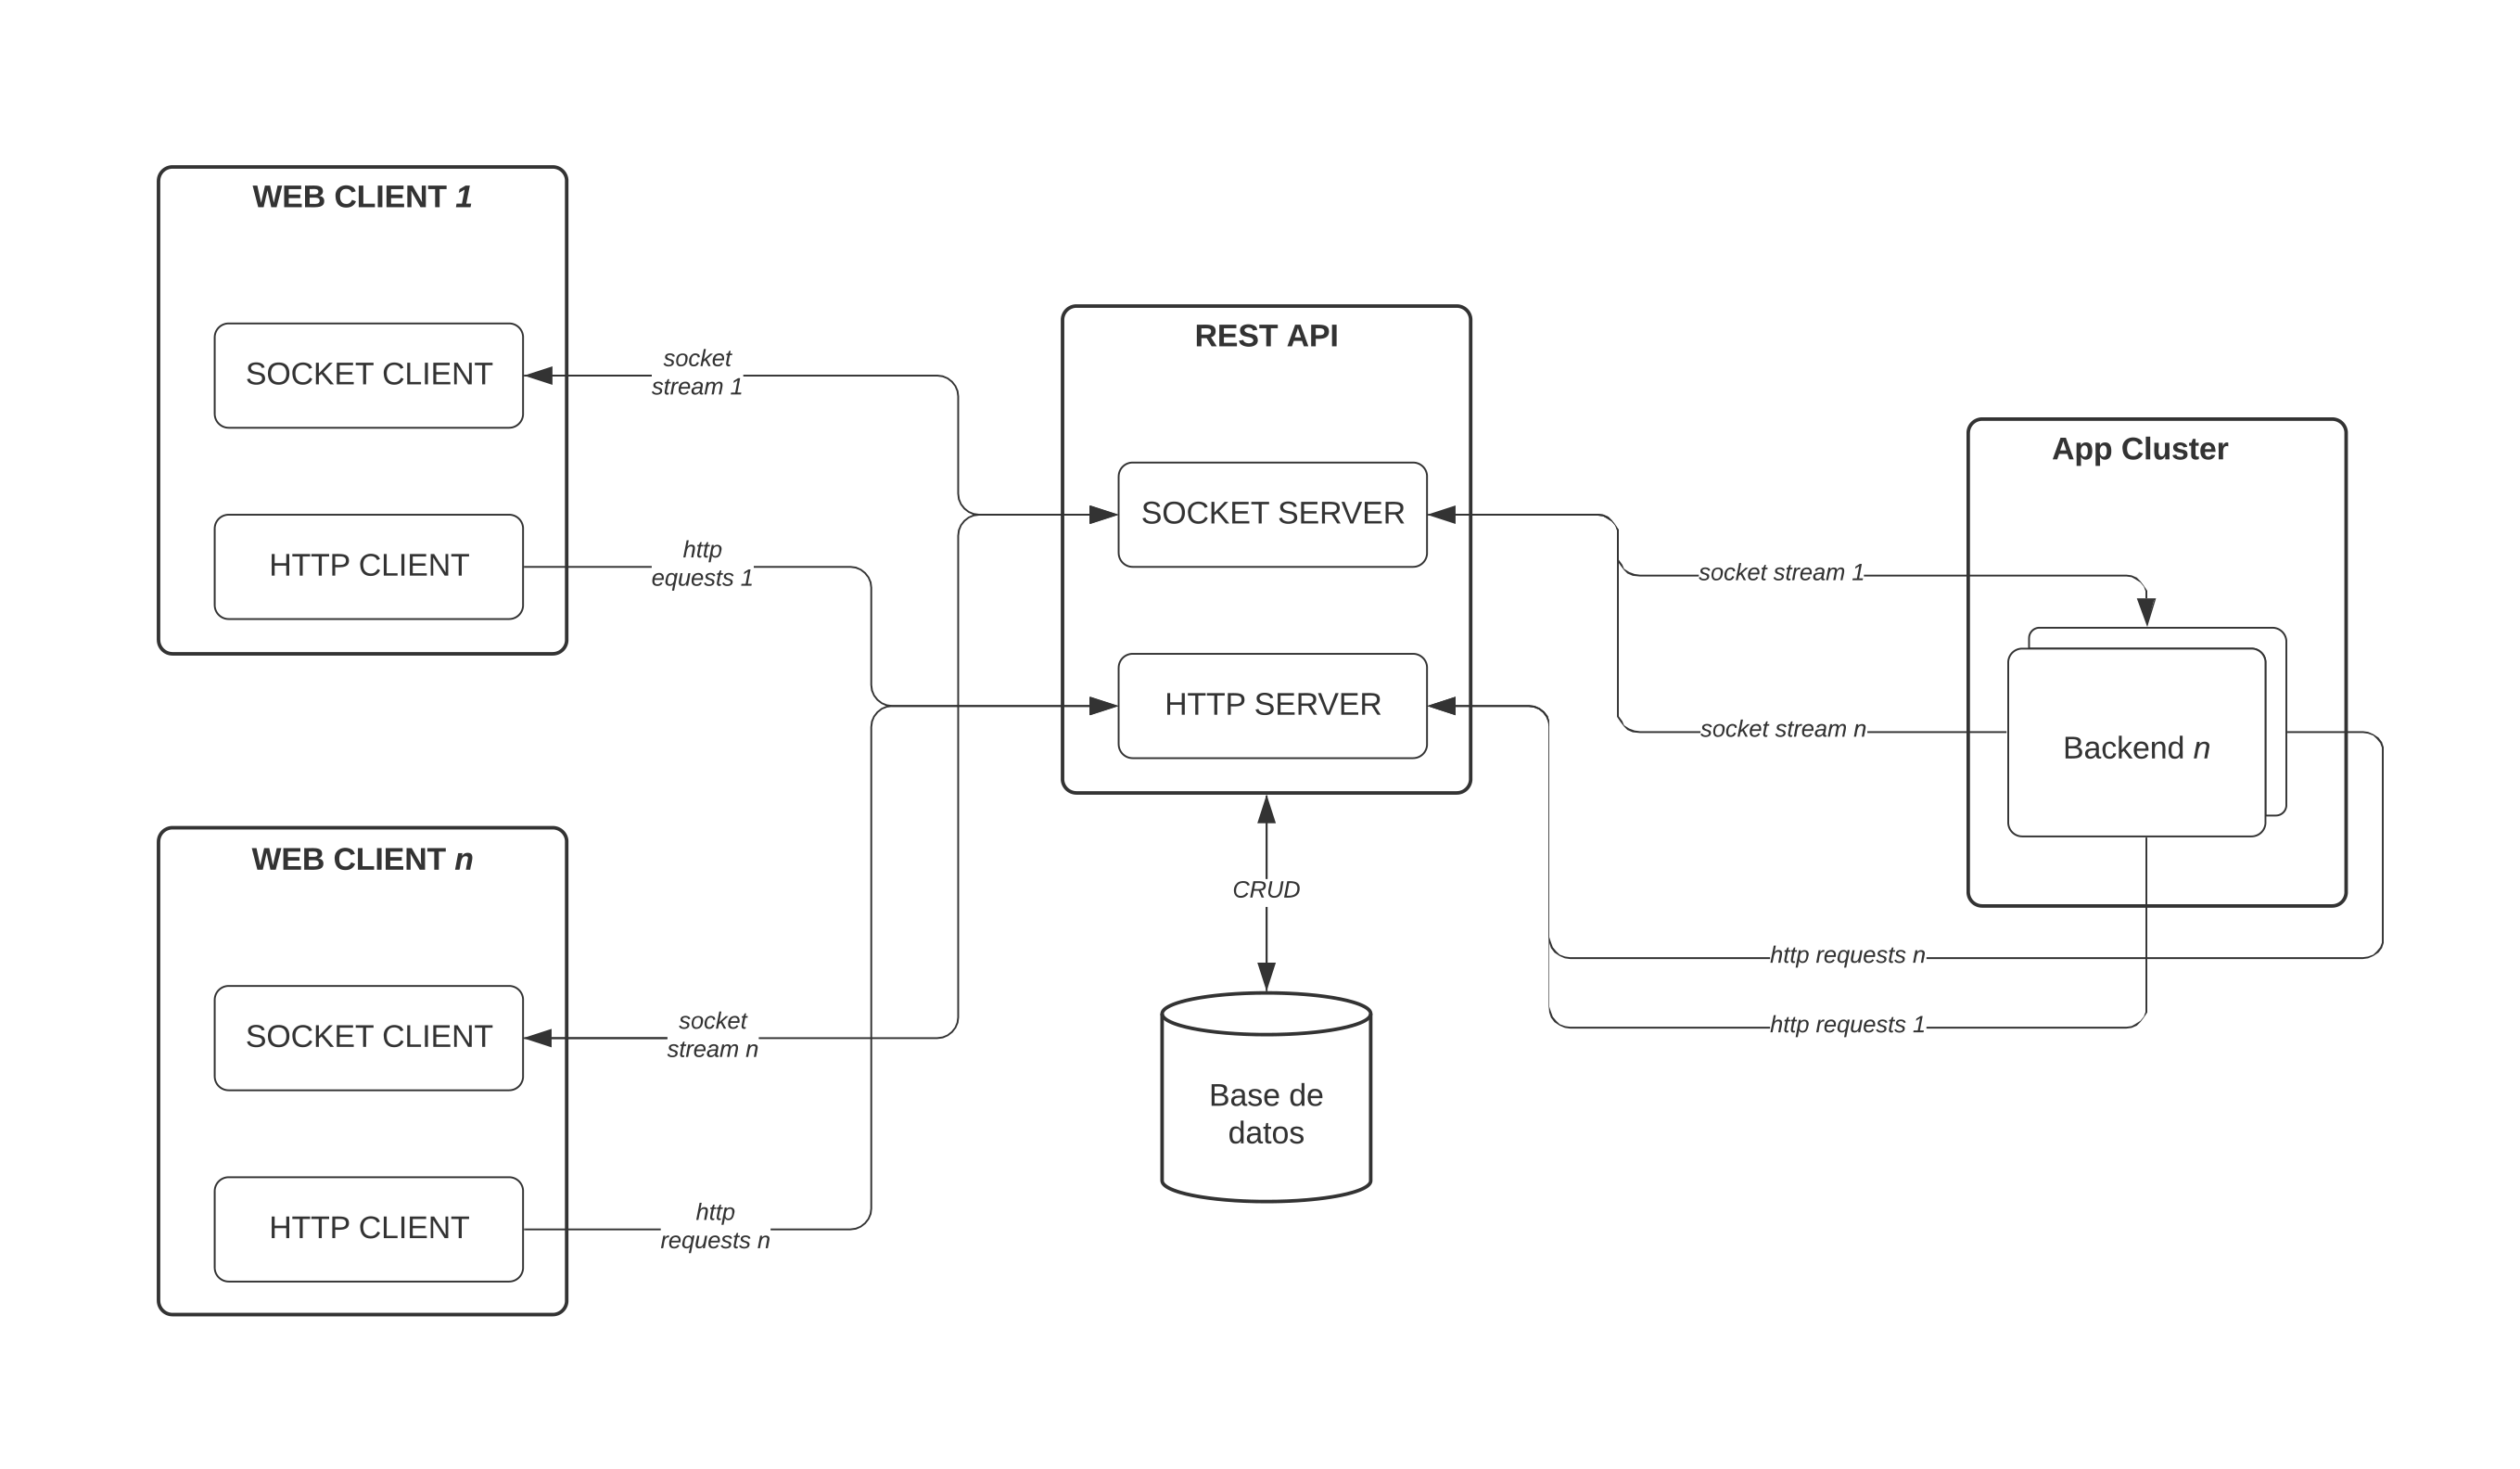
\includegraphics[scale=0.55]{seddi_diagram}}
      \caption{Esquema comunicaciones de servicios en Seddi.}
      \vspace{1.5cm}
    \end{figure}

  \egroup

  \section{Integraci\'on sobre los servicios en la nube de Seddi}
  La informaci\'on de un material para que los motores gr\'aficos del cliente web y el servicio \textit{HPC} (High-Performance Computing)
  se almacena en un \textit{TextureStack}, que son resultado de la captura \'optica de un tejido, o un SurfaceMaterial, la definici\'on para
  cualquier otro elemento de la escena 3D. Ambos motores gr\'aficos utilizan un \textit{ECS} (Entity Component System), por lo que
  la informacion sobre los materiales son una referencia un GarmentPieceComponent, en el caso de un TextureStack,
  o un MeshRenderableComponent, en el caso de un \textit{SurfaceMaterial}.\\
  Los recursos almacenan diferentes tipos de metadatos, que pueden utilizar diferentes modelos de shading, pero
  comparten la parametrizaci\'on de los materiales. En la figura 4.3 se muestran los esquemas de \'estos recursos en la
  base de datos.\\

  \begin{figure}[H]
    \vspace{0.5cm}
    \centering
      \frame{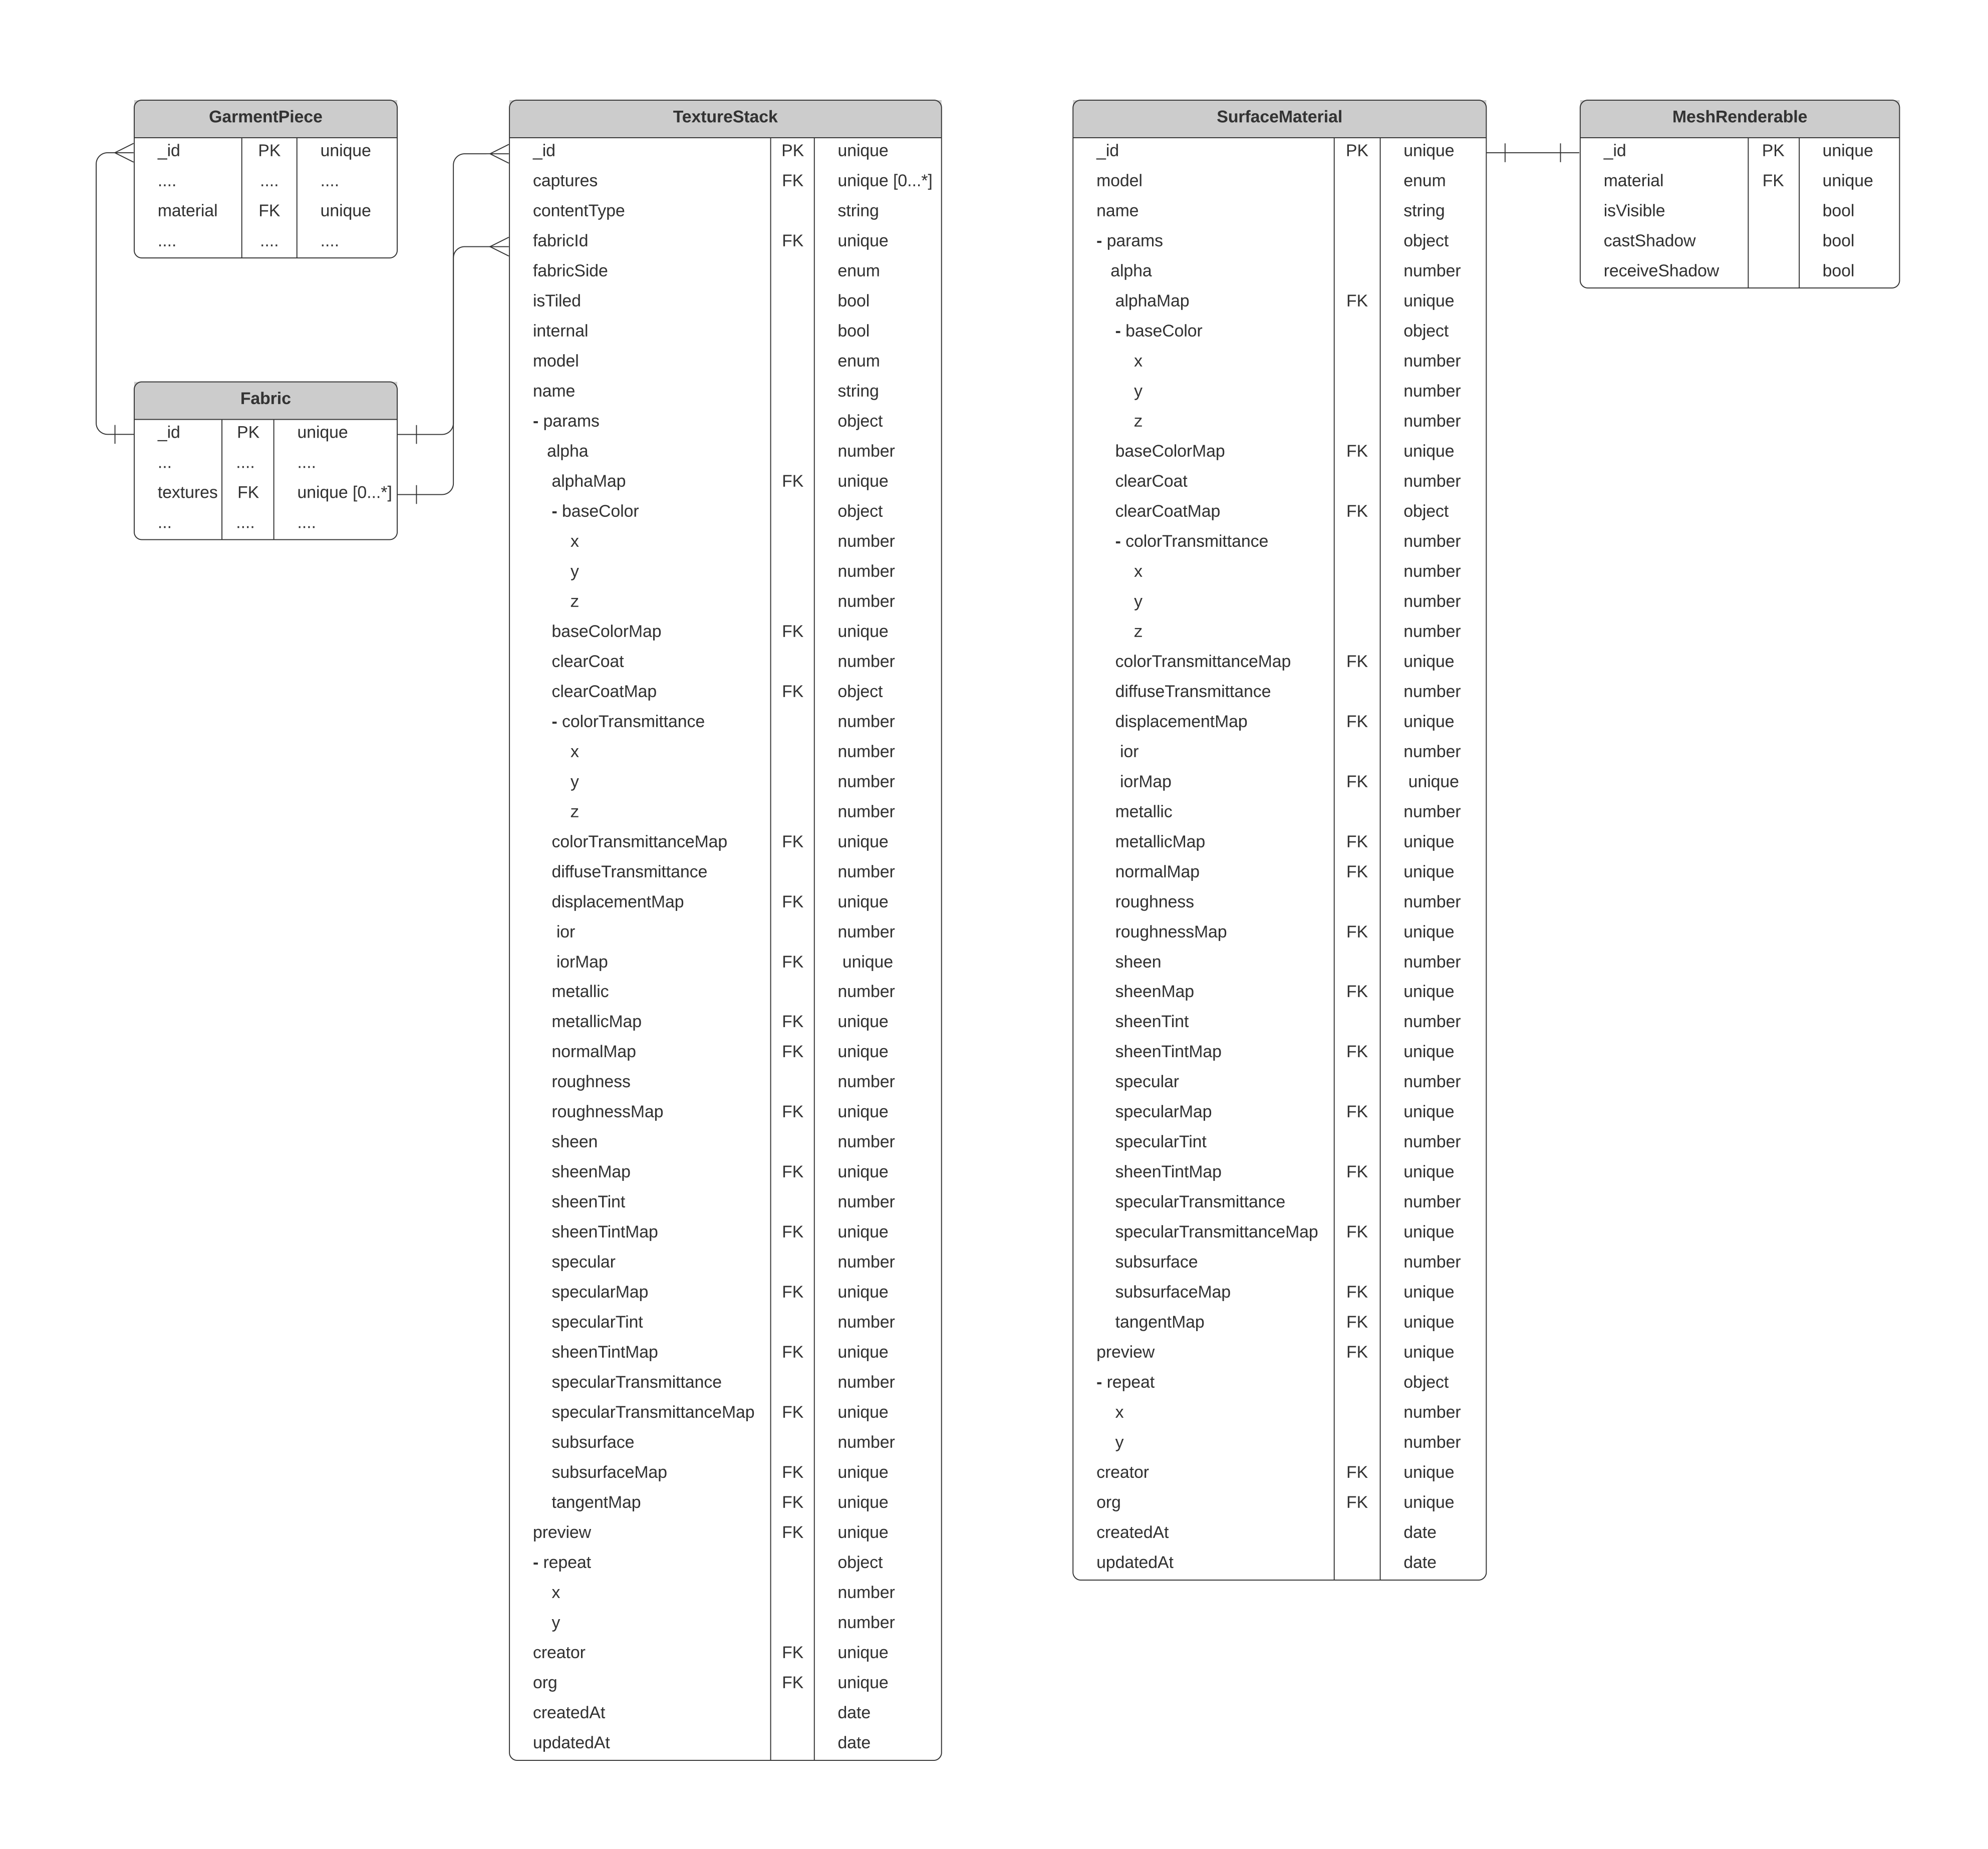
\includegraphics[scale=0.4]{materials_schema}}
    \caption{Modelo de datos de los recursos que utilizan materiales.}
    \vspace{0.5cm}
  \end{figure}
  

  El API REST es la interfaz que expone las operaciones disponible sobre cada recurso y se documentan con Swagger,
  una herramienta de documentaci\'on que sirve como gu\'ia a los desarrolladores consumidores del API. En
  la figura 4.4 se muestran la documentaci\'on sobre los tipos de peticiones y las rutas del API referidas a recursos
  SurfaceMaterial y \textit{TextureStack}.\\
  
  \begin{figure}[H]
    \vspace{0.5cm}
    \centering
      \frame{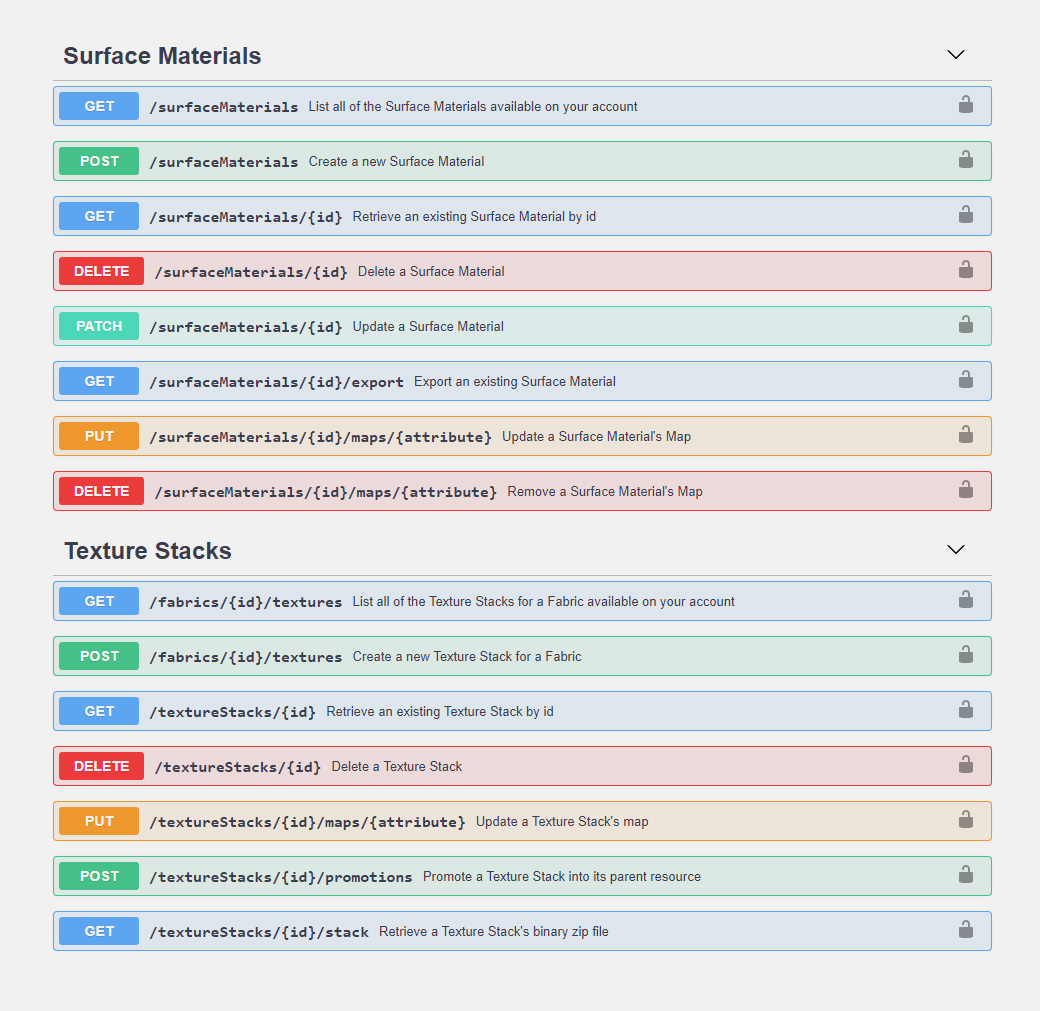
\includegraphics[scale=0.4]{swagger}}
    \caption{Documentaci\'on de los recursos SurafaceMaterial y TextureStack en Swagger.}
    \vspace{0.5cm}
  \end{figure}


  \section{Materiales PBR en ThreeJs}

  ThreeJs presenta desde su versi\'on 74 el material \textit{MeshStandardMaterial}, basado en f\'isica y desde la versi\'on
  76, el \textit{MeshPhysicalMaterial}, que extiende al anterior a\~nadiendo par\'ametros presentes en el modelo de Disney.
  El modelo est\'a basado en el de Disney 2012, pero con algunas diferencias con intenci\'on de hacerlo m\'as ligero
  para la plataforma web. A continuaci\'on se detallan los principales cambios entre los dos modelos:

    \subsection{Componente difusa}
    Al contrario que en Disney, el modelo de ThreeJs utiliza directamente el modelo de Lambert, considerando un retrodispersi\'on
    uniformemente distribuida en todas direcciones.\\

    Componente difusa en ThreeJs:

    \begin{equation}
      f_d = \frac{c}{\pi}
    \end{equation}
    \singlespacing

    Componente difusa en Disney 2012:

    \begin{equation}
      f_d = \frac{baseColor}{\pi}
      \left(  1 + (F_{D90} - 1)(1 - cos\theta_{wi})^5  \right)
      \left(  1 + (F_{D90} - 1)(1 - cos\theta_{wo})^5  \right)
    \end{equation}
    \singlespacing


    \subsection{Componente especular}
    El BRDF del l\'obulo primario es siempre isotr\'opico, a diferencia de Disney, en el que el l\'obulo primario
    puede ser isotr\'opico o anistr\'opico, no as\'i el l\'obulo de \textit{clearcoat}, que siempre es isotr\'opico.
    Adem\'as el especular utiliza un BRDF GGX, a diferencia del GTR del modelo de Disney. A continuaci\'on el c\'odigo
    del BRDF especular en ThreeJs:

    \singlespacing
    \begin{lstlisting}[caption=Clase MeshClothMaterial]
// bsdfs.glsl
// ...
vec3 BRDF_Specular_GGX(
  const in IncidentLight incidentLight,
  const in vec3
  viewDir,
  const in vec3 normal,
  const in vec3
  specularColor,
  const in float roughness
) {
  float alpha = pow2( roughness );
  vec3 halfDir = normalize( incidentLight.direction + viewDir );
  float dotNL = saturate( dot( normal, incidentLight.direction ) );
  float dotNV = saturate( dot( normal, viewDir ) );
  float dotNH = saturate( dot( normal, halfDir ) );
  float dotLH = saturate( dot( incidentLight.direction, halfDir ) );
  vec3 F = F_Schlick( specularColor, dotLH );
  float G = G_GGX_SmithCorrelated( alpha, dotNL, dotNV );
  float D = D_GGX( alpha, dotNH );
  return F * ( G * D );
}
// ...
    \end{lstlisting}
    \singlespacing

  A continuaci\'on se detallan las implementaciones de cada t\'ermino y sus cambios con respecto al modelo de ThreeJs.

    \subsubsection{T\'ermino D}
    Utiliza una aproximaci\'on de la distribuci\'on GGX, frente a la GTR utilizada en el modelo de Disney, por lo que
    presenta una cola m\'as corta.\\

    \begin{eqfloat}
      \begin{equation}
        D_{GGX}(m) = \frac{\alpha^2}{\pi((n\cdotp{m})^2(\alpha^2 - 1 ) + 1)^2}
      \end{equation}
    \caption{Funci\'on de distribuci\'on de las normales en ThreeJs}
    \end{eqfloat}
    \singlespacing

    \begin{eqfloat}
      \begin{equation}
        D_{GTR} = \frac
        {c}
        {(\alpha^2 cos^2 \theta_h + sin^2 \theta_h)^2}
      \end{equation}
    \caption{Funci\'on de distribuci\'on de las normales en Disney 2012}
    \end{eqfloat}
    \singlespacing

    \begin{lstlisting}[caption=Implementaci\'on en ThreeJs del t\'ermino de geometr\'ia]
float D_GGX( const in float alpha, const in float dotNH ) {

  float a2 = pow2( alpha );

  float denom = pow2( dotNH ) * ( a2 - 1.0 ) + 1.0; 

  return RECIPROCAL_PI * a2 / pow2( denom );

}
    \end{lstlisting}
    \singlespacing

    \subsubsection{T\'ermino F}
    Igual que en el modelo de Disney 2012, se considera la funci\'on de Fresnel-Schlick lo suficientemente precisa para
    estimar el Fresnel, sin embargo, en \'este caso se utiliza la aproximaci\'on presentada por Epic en el Siggraph de 2013.\\

    \begin{eqfloat}
      \begin{equation}
        F= F_0 + (1 - F_0)2^{(-5.55473cos\theta_d - 5.55473cos\theta_d)}
      \end{equation}
    \caption{Aproximaci\'on de la funci\'on de Fresnel en ThreeJs}
    \end{eqfloat}

    \begin{eqfloat}[!htb]
      \begin{equation}
        F= (1 - F(\theta_l) (1 - F(\theta_d)))^5
      \end{equation}
    \caption{Aproximaci\'on de la funci\'on de Fresnel en Disney 2012}
    \end{eqfloat}

    \newpage
    \begin{lstlisting}[caption=Implementaci\'on en ThreeJs de la aproximaci\'on a la funci\'on de Fresnel]
vec3 F_Schlick( const in vec3 specularColor, const in float dotLH ) {

  float fresnel = exp2( ( -5.55473 * dotLH - 6.98316 ) * dotLH );

  return ( 1.0 - specularColor ) * fresnel + specularColor;

}
    \end{lstlisting}
    \singlespacing

    \subsubsection{T\'ermino G}
    Para definir las microfacetas en sombra o enmascaradas, ThreeJs utiliza el mismo t\'ermino que Disney 2012, usa
    la formulaci\'on de Smith para separar la funci\'on en dos componentes, luz y vista, utilizando la misma ecuaci\'on
    para las dos.\\

    $$
    G(w_i, w_o) = \frac{0.5}{G_1(w_i) + G_1(w_o)}
    $$
    \singlespacing
    $$
    G_1(w_i) = (n \cdot{w_o}) \sqrt{((-n\cdot{w_i}) \alpha^2 + n\cdot{w_i}) n\cdot{w_i} + \alpha^2}
    $$
    \singlespacing
    $$
    G_1(w_o) = (n \cdot{w_i}) \sqrt{((-n\cdot{w_o}) \alpha^2 + n\cdot{w_o}) n\cdot{w_o} + \alpha^2}
    $$
    % float Lambda_GGXV = NdotL * sqrt (( - NdotV * alphaG2 + NdotV ) * NdotV + alphaG2 );
    \begin{eqfloat}[!htb]
      \begin{equation}
        \textrm{siendo}\ k = \frac{(roughness + 1)^2}{8}
      \end{equation}
    \caption{Funci\'on de geometr\'ia en ThreeJs}
    \end{eqfloat}
    \singlespacing

    $$
    G(w_i, w_o) = G_1(w_i)G_1(w_o)
    $$

    \begin{eqfloat}[!htb]
      \begin{equation}
        G_1(w_o) = \frac{n\cdot{w_o}}{(n\cdot) (1 - k) + k}
      \end{equation}
    \caption{Funci\'on de geometr\'ia en Disney 2012}
    \end{eqfloat}
    \singlespacing

  \begin{lstlisting}[caption=Clase MeshClothMaterial]
float G_GGX_SmithCorrelated( const in float alpha, const in float dotNL, const in float dotNV ) {

  float a2 = pow2( alpha );

  // dotNL and dotNV are explicitly swapped. This is not a mistake.
  float gv = dotNL * sqrt( a2 + ( 1.0 - a2 ) * pow2( dotNV ) );
  float gl = dotNV * sqrt( a2 + ( 1.0 - a2 ) * pow2( dotNL ) );

  return 0.5 / max( gv + gl, EPSILON );

}
  \end{lstlisting}

    \subsection{Clearcoat}
    El efecto de \textit{clearcoat}, se utiliza para simular efectos de barniz o recubrimientos, y se aplican tanto en Disney
    2012 como un l\'obulo secundario. Mientras que en ThreeJs se utiliza el mismo BRDF con la misma parametrizaci\'on que para
    el l\'obulo primario, en Disney 2012, var\'ia la parametrizaci\'on de los t\'erminos D y G.\\

    $$
    G_{GGX}(v) = \frac
    {2 (n \cdot{v})}
    {(n \cdot{v}) + \sqrt{ \alpha^2 + (1 - \alpha)^2 (n \cdot{v})^2 }}
    $$
    \begin{eqfloat}[!htb]
      \begin{equation}
      \textrm{siendo}\ \alpha=0.25,\;
      G_{GGX}(v) = \frac
      {2 (n \cdot{v})}
      {(n \cdot{v}) + \sqrt{ 0.0625 + 0.5625 (n \cdot{v})^2 }}
      \end{equation}
    \caption{Funci\'on de geometr\'ia para el l\'obulo de \textit{clearcoat} en Disney 2012}
    \end{eqfloat}
    \singlespacing

    $$
    D_{GTR} = \frac
    {c}
    {(\alpha^2 cos^2 \theta_h + sin^2 \theta_h)^\gamma}
    $$
    \begin{eqfloat}[!htb]
      \begin{equation}
      \textrm{siendo}\ \gamma=1.0,\;
      D_{GTR} = \frac
      {c}
      {(\alpha^2 cos^2 \theta_h + sin^2 \theta_h)}
      \end{equation}
    \caption{Funci\'on de distribuci\'on de las normales para el l\'obulo de \textit{clearcoat} en Disney 2012}
    \end{eqfloat}
    \singlespacing
    
    \subsection{Sheen}
    El par\'ametro de sheen ofrece un mayor control sobre la reflectancia especular, permitiendo crear materiales con
    especulares en dos tonos. Mientras que ThreeJs utiliza un BRDF diferente cuando el par\'ametro de sheen, en el
    BRDF de Disney 2012 el \textit{sheen} se modela como otro l\'obulo adicional.\\
    \todo[inline]{A\~nadir f\'ormulas}

  \section{Arquitectura del motor de renderizado de ThreeJs}
  El nuevo material extender\'a la librer\'ia de materiales para ofrecer una interfaz igual al resto de materiales nativos
  de ThreeJs. Para ello, estudiaremos la arquitectura del motor de renderizado de ThreeJs tomando como referencia los dos
  materiales disponibles en la librer\'ia, \textit{MeshStandardMaterial} y \textit{MeshPhysicalMaterial}.

  \begin{figure}[H]
    \centering
      \frame{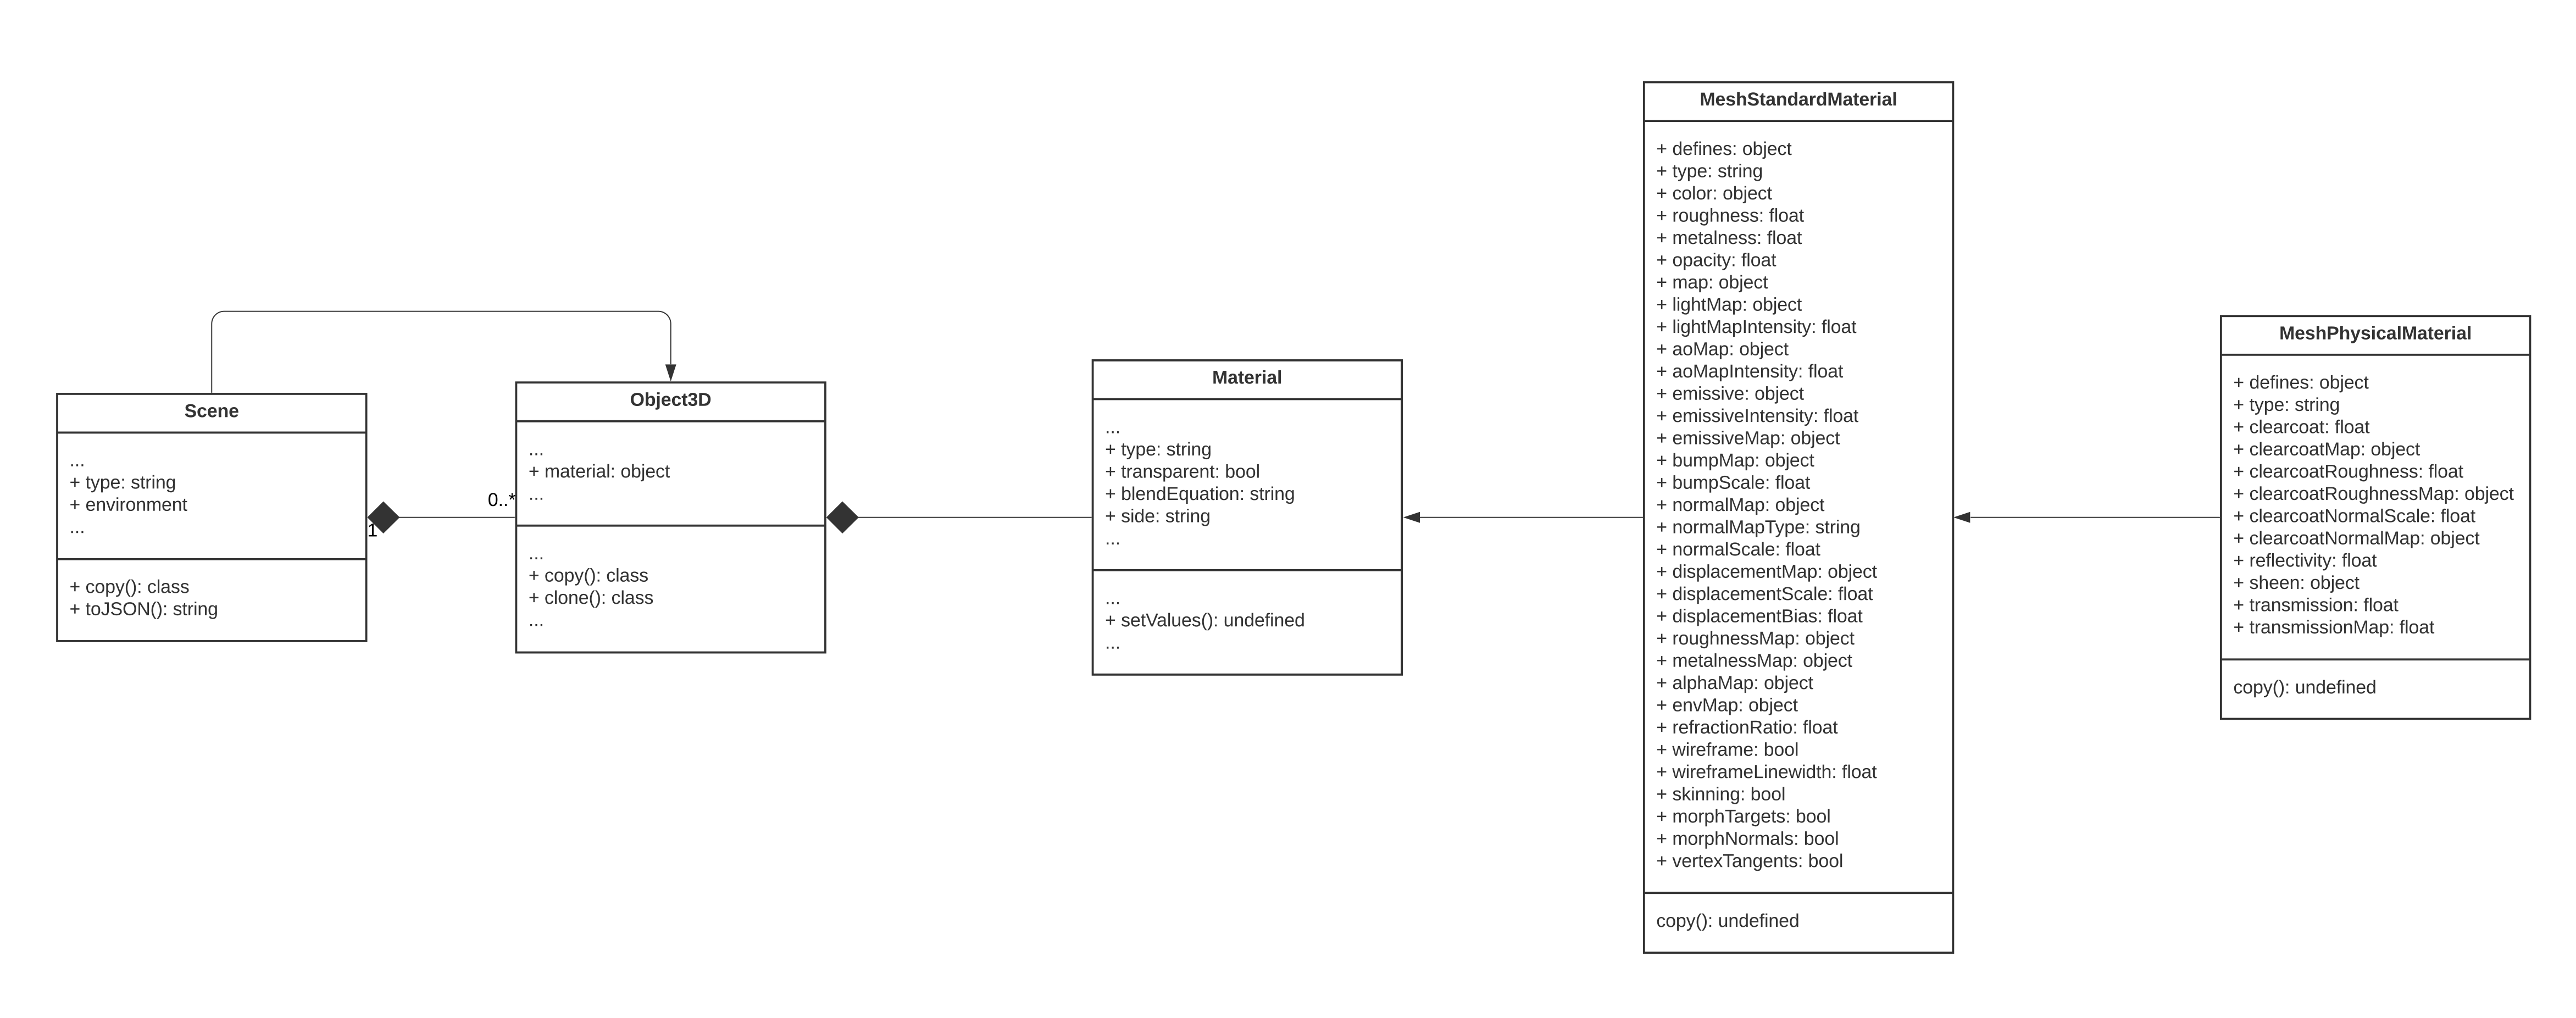
\includegraphics[scale=0.35]{threejs_scenegraph}}
    \caption{Documentaci\'on de los recursos SurfaceMaterial y TextureStack en Swagger.}
    \vspace{0.5cm}
  \end{figure}

  La clase base de la que heredan es \textit{Material} y almancena informaci\'on b\'asica de
  cualquier tipo de material: opacidad, ecuaci\'on de blending, la cara visible, etc. Adem\'as proporciona un m\'etodo
  para configurar los valores de las propiedades del material, as\'i como m\'etodos para la copia, clonado o serializaci\'on
  del material.\\

  \textit{MeshStandarMaterial} hereda de \textit{Material} y es el shader base de un material PBR. Almacena propiedades comunes
  como el color el mapa de normales, mapa de desplazamiento, adem\'as de sobreescribir el objeto de \textit{defines} y el tipo
  de material. Adem\'as sobreescribe la funci\'on de \textit{copy} de la clase \textit{Material} para copiar correctamente
  estas nuevas propiedades.\\
  % \todo[inline]{\hspace*{1.5em}El \textit{MeshPhysicalMaterial} hereda de \textit{MeshStandarMaterial} y es el shader base de un material PBR. Almacena propiedades comunes
  % como el color el mapa de normales, mapa de desplazamiento, adem\'as de sobreescribir el objeto de \textit{defines} y el tipo
  % de material. Adem\'as sobreescribe la funci\'on de \textit{copy} de la clase \textit{Material} para copiar correctamente
  % estas nuevas propiedades.}

  El \textit{MeshPhysicalMaterial} hereda de \textit{MeshStandarMaterial} an\~adiendo el l\'obulo de \textit{clearcoat} y
  el BRDF alternativo para el \textit{sheen}, utiliza sus propios \textit{defines} y sobreescribe la funci\'on de copia.\\

  Los elementos que se renderizan en la escena, heredan de la clase base \textit{Object3D}, que guarda una referencia
  al material. El grafo de escena se gestiona desde la clase \textit{Scene}, que hereda de \textit{Object3D} y guarda
  informaci\'on sobre el fondo o mapa de entorno, adem\'as de proporcionar sus propios m\'etodos de copia y serializaci\'on
  a JSON.

  \begin{figure}[H]
    \vspace{0.5cm}
    \centering
      \frame{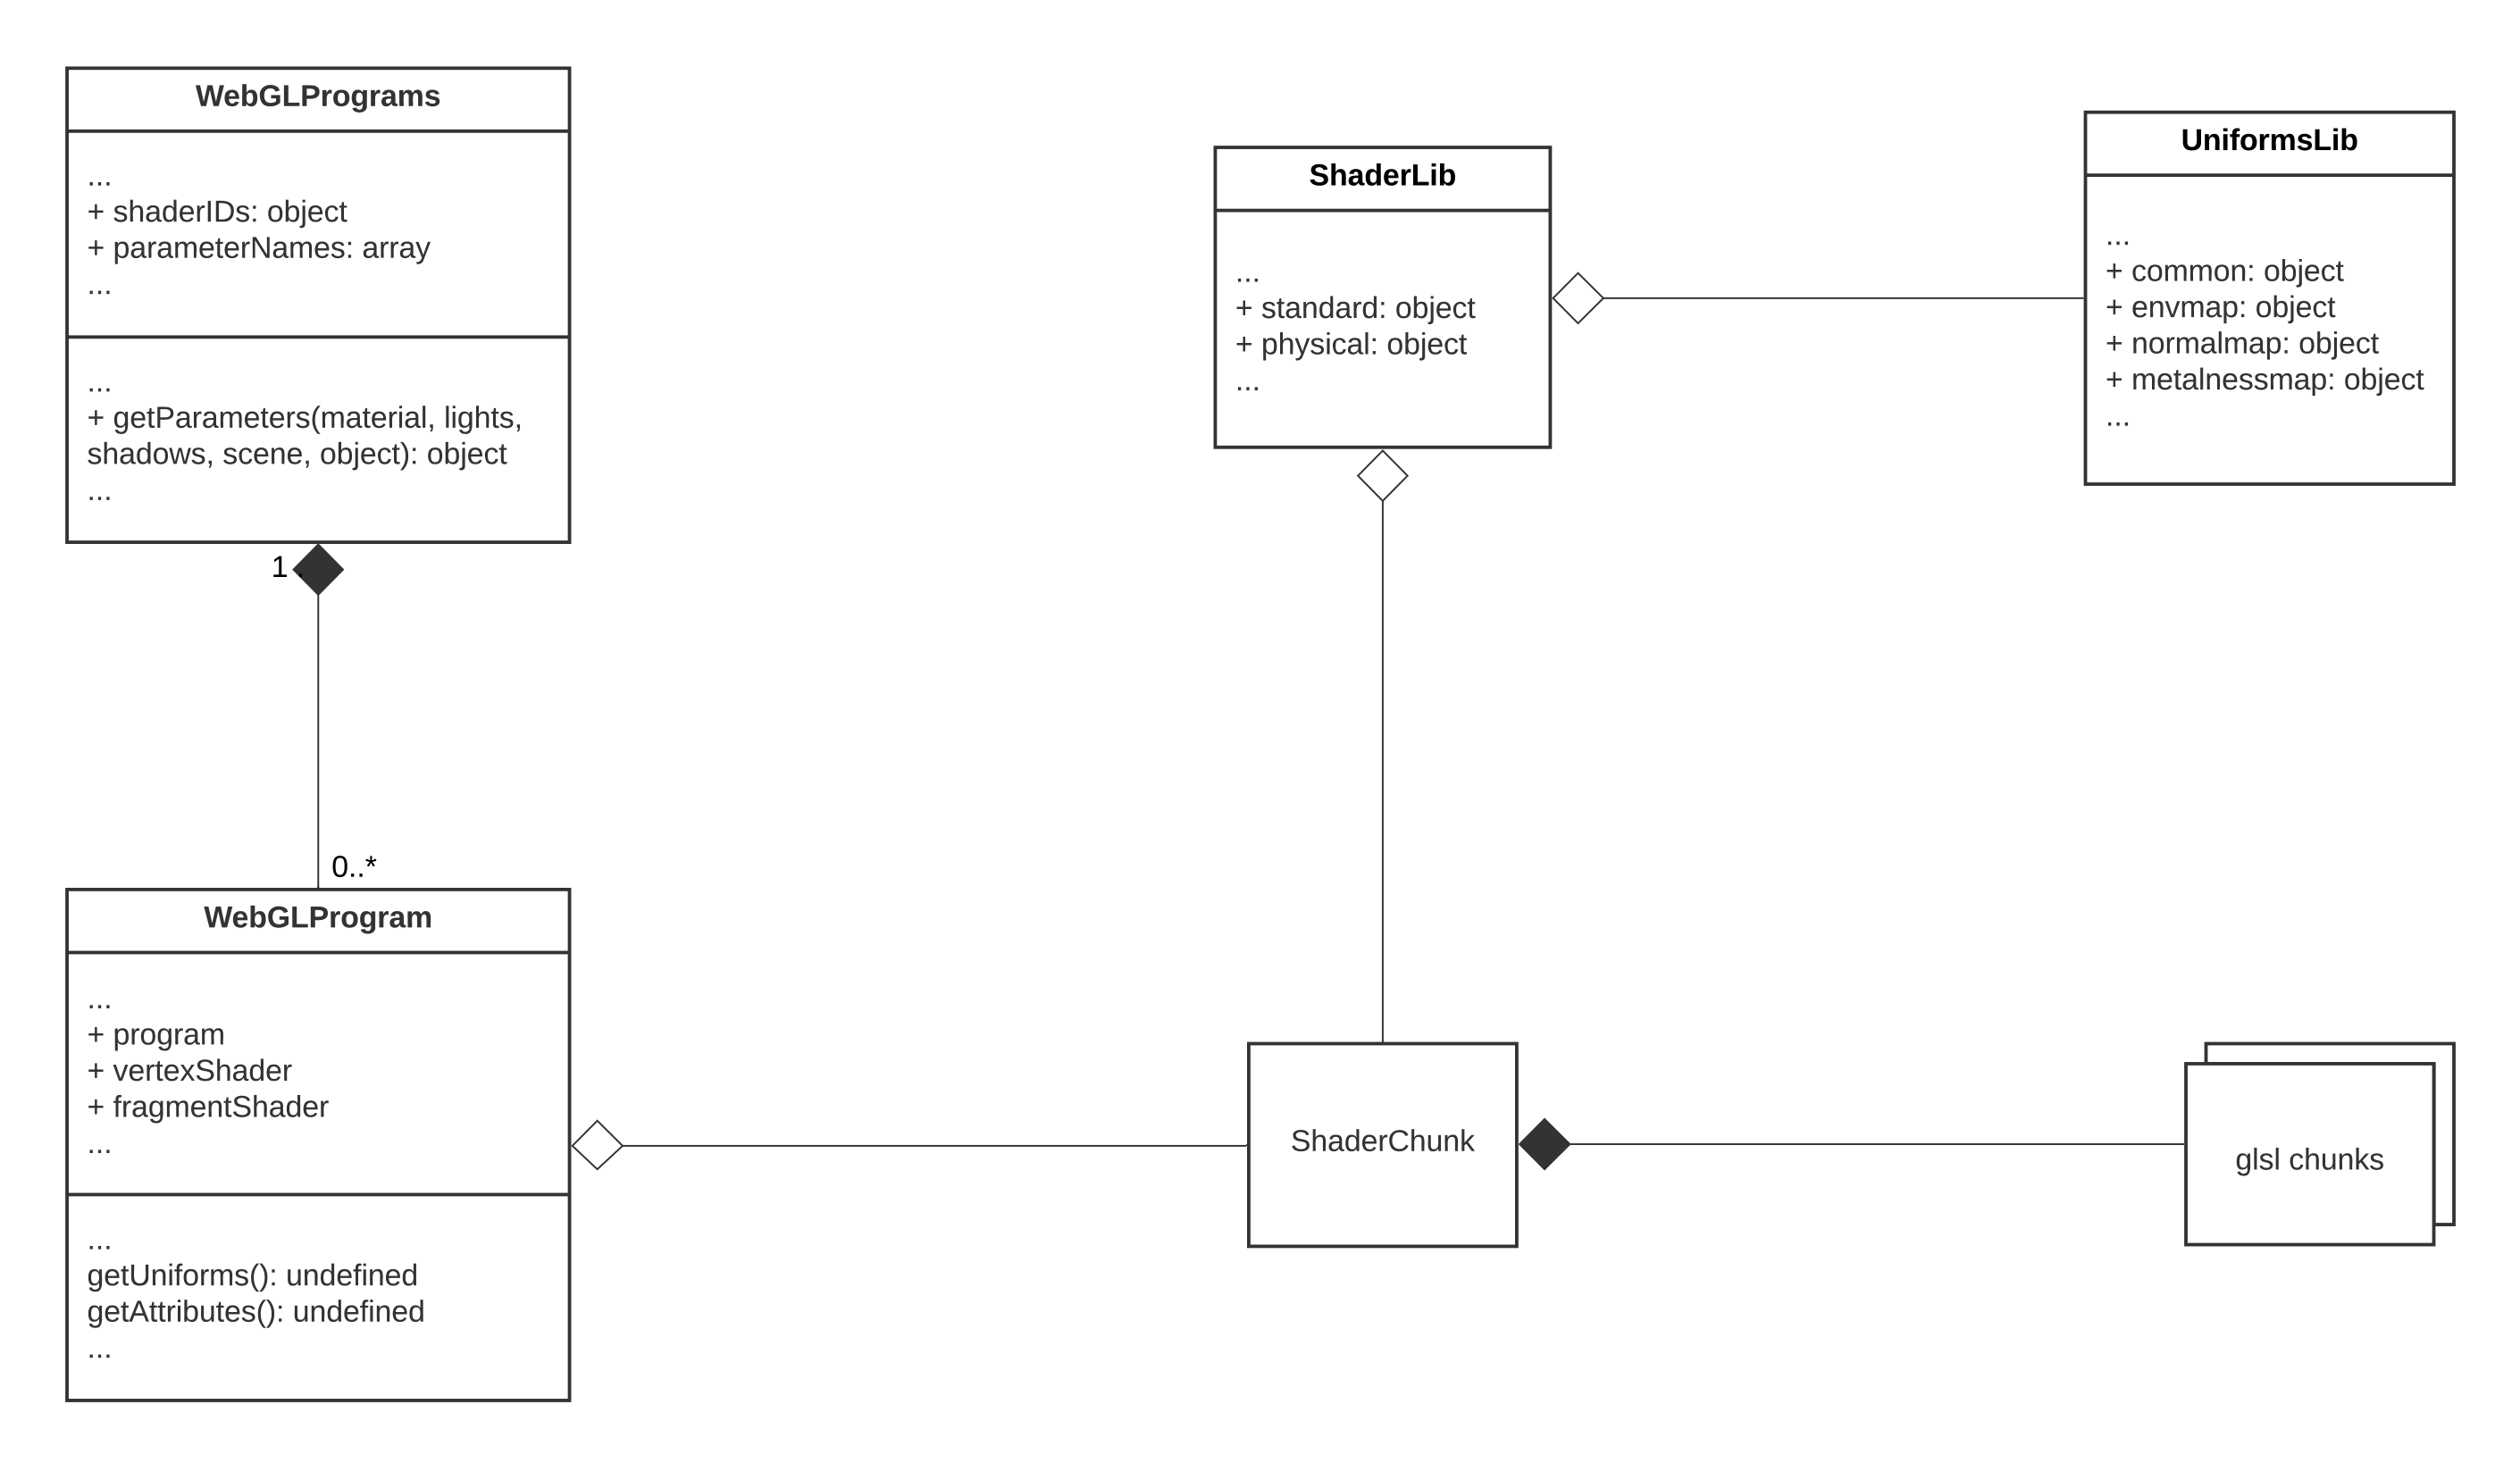
\includegraphics[scale=0.37]{threejs_webglprogram}}
    \caption{Estructuras de datos de ThreeJs que se encargan de la gesti\'on de programas de WebGL}
  \end{figure}

  Para generar los WebGLProgram del API de WebGL, ThreeJs organiza el c\'odigo GLSL en \textit{chunks}, o trozos de c\'odigo
  que se reutilizan y se componen en tiempo de ejecuci\'on para generar el c\'odigo del programa de WebGL. De la misma forma, los
  \textit{uniforms} que se reutilizan entre programas se organizan en el objeto \textit{UniformsLib}. El objeto ShaderLib almacena
  los materiales est\'andar de la librer\'ia, \textit{MeshStandardMaterial}, \textit{MeshPhysicalMaterial}, etc, utilizando los trozos
  de c\'odigo GLSL de \textit{ShaderChunk}, los uniforms definidos en \textit{UniformsLib}, adem\'as de los \textit{uniforms} \'unicos
  para cada tipo de material.
  La clase \textit{WebGLProgram} se encarga de juntar los trozos de c\'odigo GLSL y generar la cadena de texto que se utilizar\'a en
  el programa WebGL. Las instancias de la clase \textit{WebGLProgram} se cachean en una lista de referencias en el closure \textit{WebGLPrograms}, que proporciona
  acceso a la lista, as\'i como funciones para actualizarla u obtener los par\'ametros o los \textit{uniforms} de un programa. \\


  \begin{figure}[H]
    \vspace{0.5cm}
    \centering
      \frame{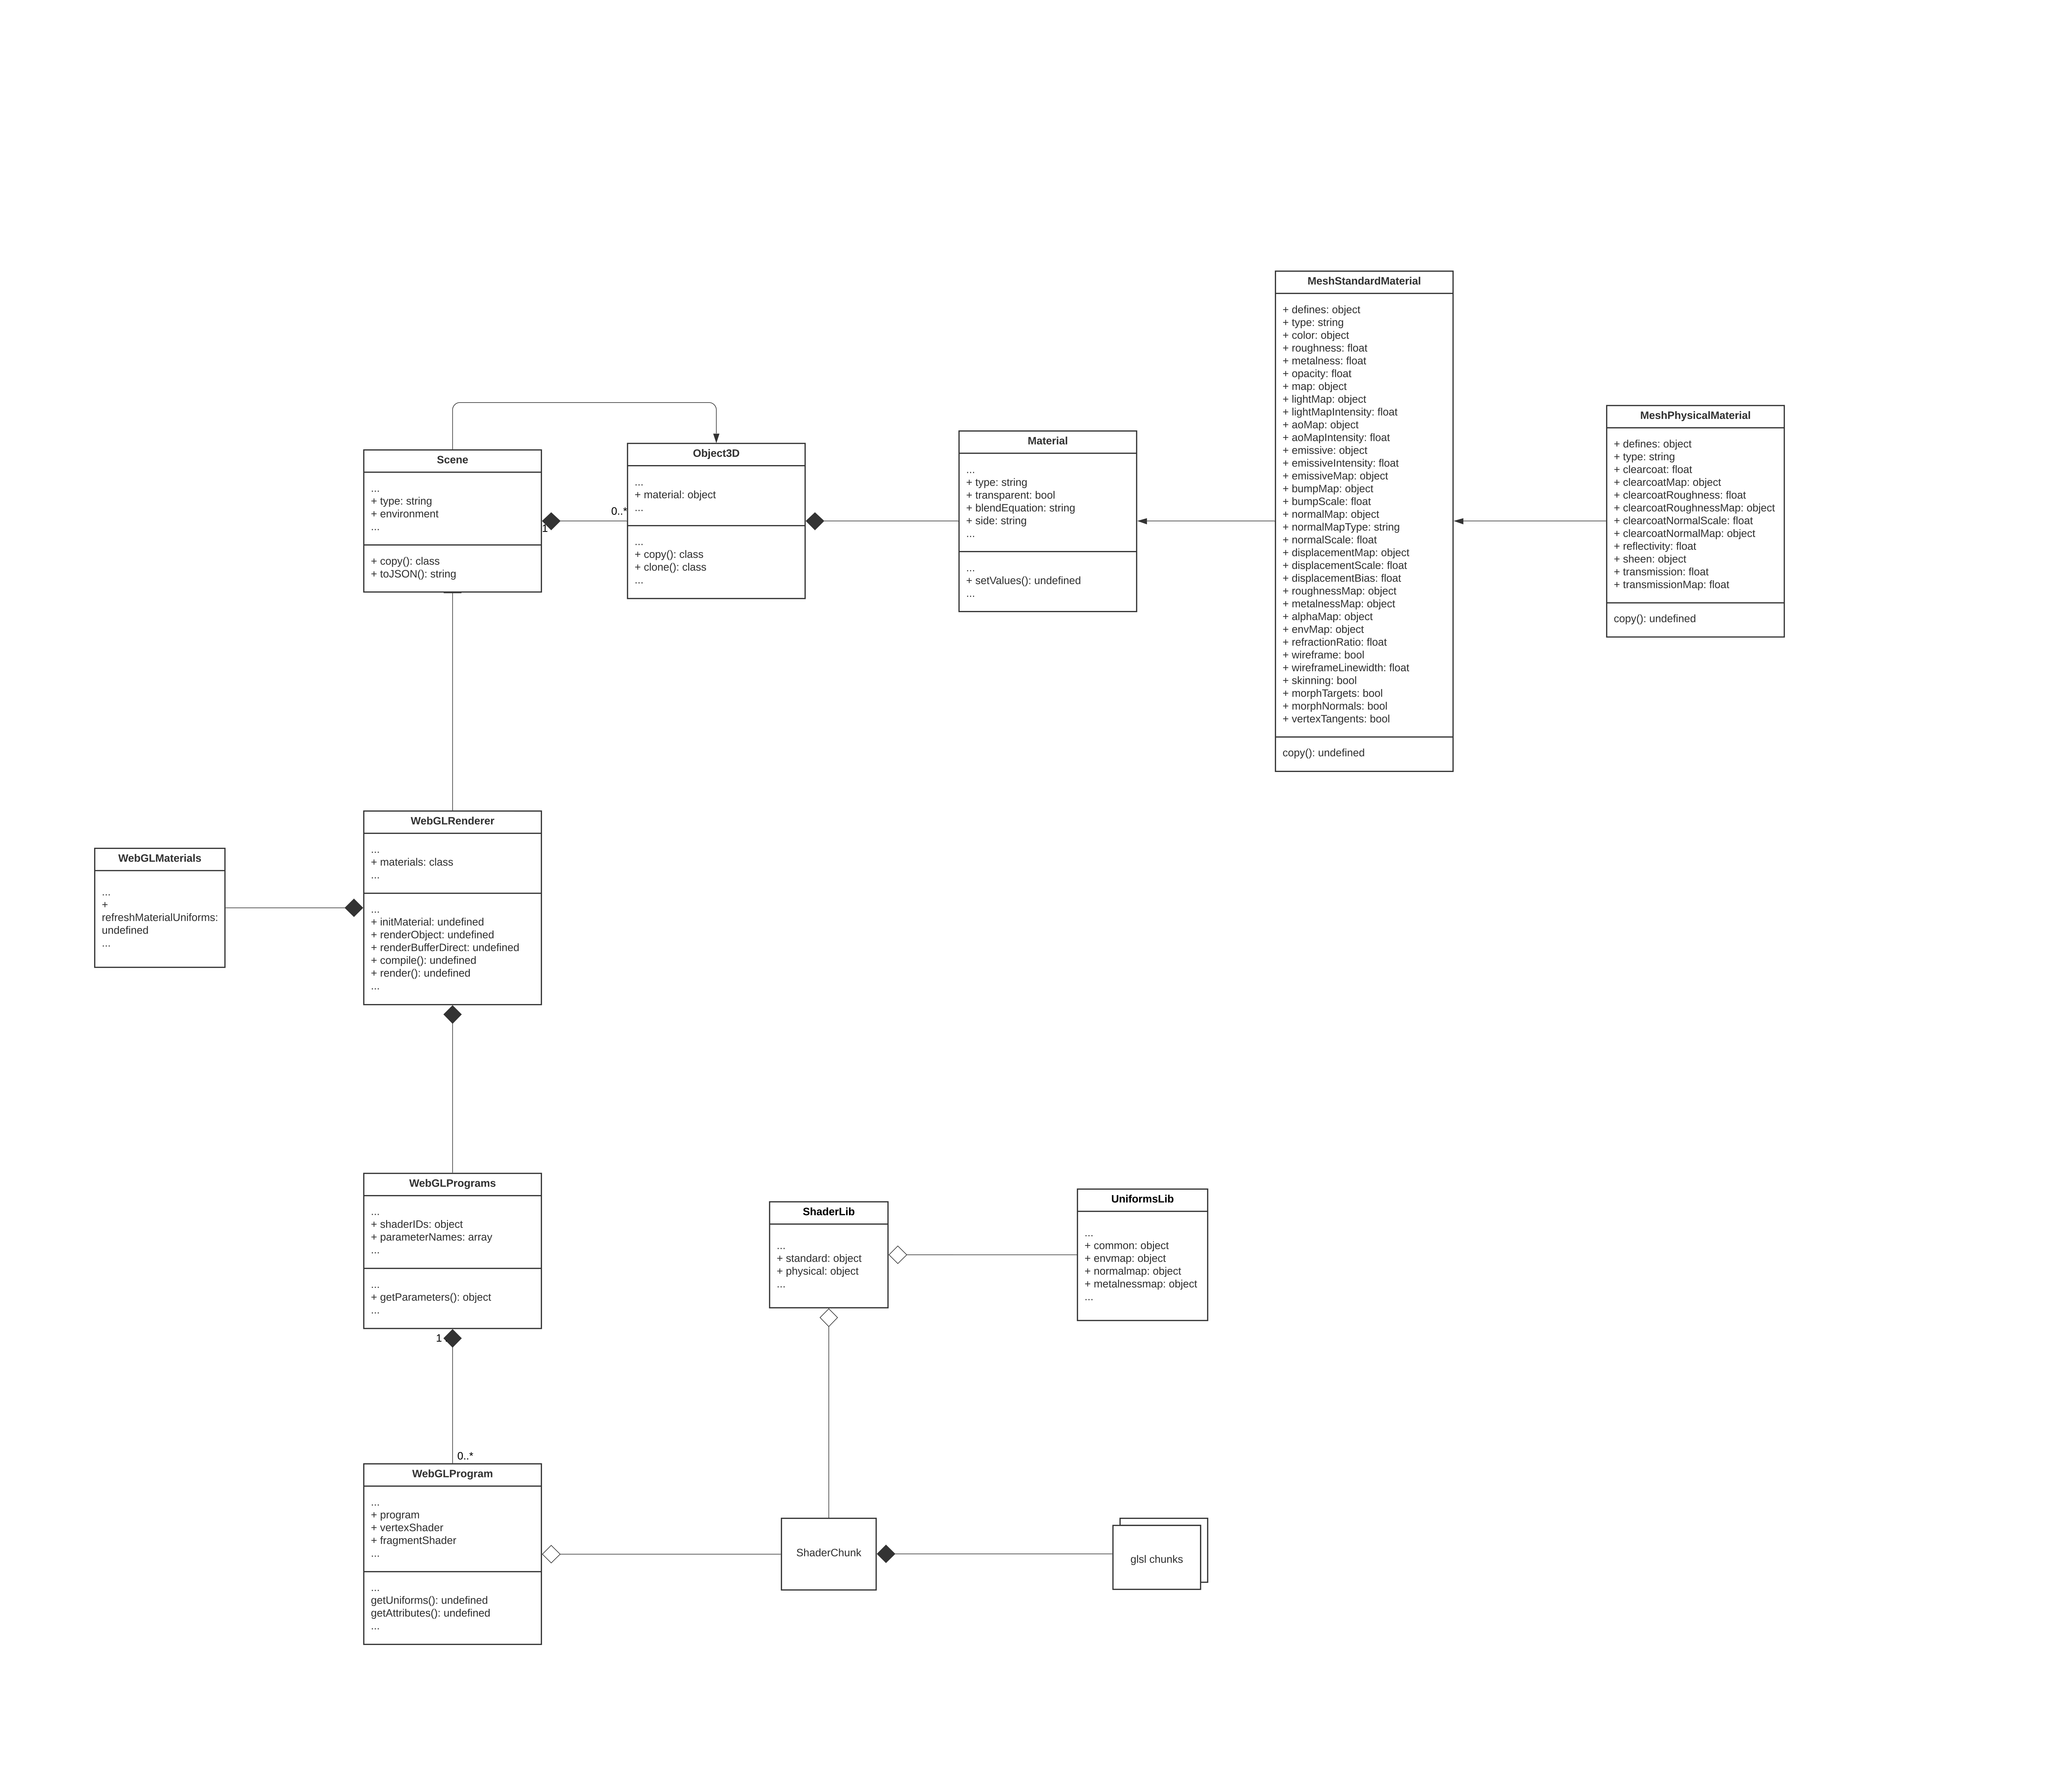
\includegraphics[scale=0.26]{threejs_renderer_architecture.png}}
    \caption{Diagrama de clases del motor de renderizado de ThreeJs.}
    \vspace{0.5cm}
  \end{figure}

  La clase WebGLRenderer es donde se gestiona la l\'ogica del motor de render y se orquesta la relaci\'on entre todos estos componentes.
  WebGLRenderer recibe una referencia al grafo de escena, la clase Scene, que se encarga de inicializar y actualizar todos
  los materiales de la escena, referenciados en la clase base de cualquier elemento que se renderiza en la escena, Object3D.
  Tiene una referencia al closure WebGLMaterials, que ofrece un m\'etodo para actualizar los \textit{uniforms} de cualquier tipo
  de los materiales nativos de ThreeJs.

  % Todos los programas GLSL se gestionan desde WebGLPrograms, un closure que contiene un lista de \textit{ids} de los materiales
  % nativos de la librer\'ia y otra lista de todos los posibles par\'ametros de \'estos materiales. Cachea los programas utilizados
  % en la aplicaci\'on y propociona m\'etodos para obtener los par\'ametros de un material, obtener sus uniforms, cachear un programa,
  % obtener un programa o generarlo en caso de que no exista, o borrarlo. WebGLPrograms almacena instancias de la clase WebGLProgram